%\section{NI InsightCM Enterprise for Condition Monitoring}
\section{Condition Monitoring Tools}

There are many commercial tool offerings for machine condition monitoring.
Major players in the marketplace include Br\"{u}el \& Kj{\ae}r Vibro, ClampOn AS, Data Physics Corporation, DLI Engineering Corp, Emerson Process Management, FLIR Systems Inc., GE Energy, Honeywell Process Solutions, among others \cite{ResarchandMarkets15}. 
We now introduce one such MCM tool; 
National Instruments' (NI) InsightCM\textsuperscript{TM} Enterprise~\cite{InsightCMBrochure15}. 
InsightCM is an online MCM tool for monitoring 
%acquires and analyzes sensory information, generates alarms, allows maintenance specialists to %visualize and manage data, and simplifies deployment of large numbers of monitoring systems. It 
health of critical rotating machinery and auxiliary rotating equipment. The goal is to optimize machine performance, maximize up-time, reduce maintenance costs, and increase safety.
This solution allows maintenance specialists to
acquire, analyze, visualize, and manage sensor data throughout the life cycle to draw diagnostic conclusions, manage alarms based on calculated features and sensor measurements,
remotely configure, monitor, and manage acquisition devices, as well as
authenticate users and devices to address network security concerns. By integrating into the IT infrastructure the tool can interact with existing databases and enterprise software. 

Figure~\ref{fig:insightcm-architecture} illustrates key components of the InsightCM solution: monitoring systems, server for data management and analysis, data explorer clients, and management infrastructure.

\begin{figure}[ht]
    \centering
    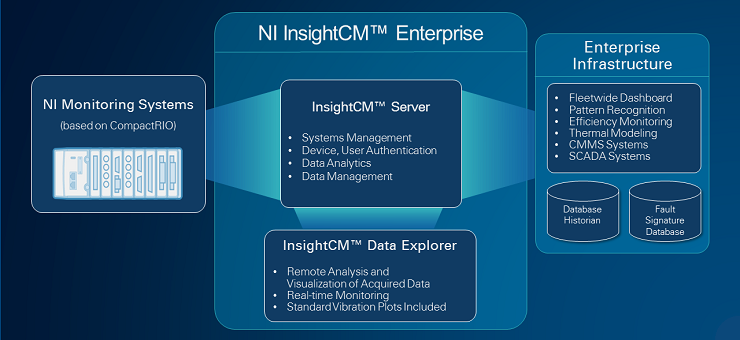
\includegraphics[width=.8\textwidth]{InsightCM_Architecture}
    \caption{NI Insight\textsuperscript{TM} Architecture}
    \label{fig:insightcm-architecture}
\end{figure}

%With the InsightCM Enterprise solution (Figure~\ref{fig:insightcm-architecture}), data is automatically acquired using CompactRIO-based NI Condition Monitoring Systems, and transmitted to the server where it is stored \cite{ni_crio}. 
%The NI InsightCM Server software calculates condition indicators and manages the CompactRIO systems. 
%The data is then avaialable for remote viewing and analysis using the NI InsightCM Data Explorer client application. 
%Data is also exportable as tags to third-party software packages running at the enterprise IT level.

%NI InsightCM\textsuperscript{TM} Enterprise solution consists of four main components (Figure~\ref{fig:insightcm-architecture}): \emph{CompactRIO-based NI Condition Monitoring Systems}, \emph{InsightCM\textsuperscript{TM} Data Explorer}, \emph{InsightCM\textsuperscript{TM} Server} and interface with existing enterprise architecture.


The monitoring devices at the edges of the system are NI CompactRIO platforms \cite{ni_crio}.
These devices, in addition to sensors and I/O modules, have processing and reconfigurable components for inline data processing, control analytics, network communication, and timing.
The CompactRIO devices supports a range of analog and digital sensors, such as proximity probes, accelerometers, pressure sensors, voltage and current sensors, thermocouples, and temperatur detectors. 
%Data is automatically acquired and transmitted to the server where it is stored. 
The monitoring system supports periodic monitoring as well as observation of important transient events such as start-ups and coast-downs. 
The {\em periodic recorder mode} allows data logging based on configurable time intervals, measurements, and user triggers. 
Dynamic waveform and static measurement sensors account for 80\% of measurements in a predictive maintenance program, suitable for replacing traditional, manual diagnostic rounds. 
The {\em transient recorder mode} streams time waveform data during transient events at run-up and coast-down until steady state is maintained, and includes support for accelerometers, velocity meters, and proximity probes. 

%NI InsightCM\textsuperscript{TM} S
The server delivers 
%in-motion -- what is in-motion analytics?
analytics coupled with management of CompactRIO systems, data, and alarms. The server software manages reliable, loss-less communication across the entire architecture and includes capabilities to configure, view, and manage the remote acquisition systems. 
The software processes dynamic waveform data and analyzes RMS, peak-peak, true-peak, derived-peak, DC gap, crest factor, and spectral bands. It also supports custom measurements like bearing, gear, and other fault frequencies. Additionally, the server provides a security layer to authenticate and protect sensor and server data.

%NI InsightCM\textsuperscript{TM} Data Explorer provides 
The data explorer provides
%in-depth, -- sounds like a marketing term - unnecessary?
interactive visualization and analysis of real-time and historical offline data stored in the server. The software package helps in remotely analyzing raw time-series data and results, drawing comparisons and viewing historical trends with support for standard vibration plots. The data explorer provides two modes: one for viewing periodically acquired data and one for viewing previously captured transient events. Users can detect imbalances, bent shafts, misalignment, bearing defects, and other faults in rotating machinery, and determine actions that need to be taken as part of diagnosis and maintenance procedures.

InsightCM has been widely used across multiple industrial domains including traditional power generation, oil and gas, renewable power generation, transportation and aerospace, heavy equipment, and manufacturing~\cite{MCM_UC_NI}. We discuss the use of InsightCM for a power grid monitoring application.

Duke Energy \cite{dukewebsite} is the largest power generation holding company in the US with a diversified energy portfolio mix and the capability to generate 58GW across 80 plants. Data used to be collected manually in periodic rounds on assets such as turbines, transformers, boilers, radiators, valves, motors, pumps, fans, and generators. The typical measurements include motor current, lube oil level, vibration, pressure, performance, and thermography. In this approach, 80\% of the effort was spent on data collection, and 20\% on analytics. Besides being labor intensive (about 60000 rounds/month), this approach has limited instrumentation and inconsistent diagnostics, which severely constrains the analysis.
By employing InsightCM for condition monitoring, Duke Energy was able to phase out manual collection and spend more resources on the analysis. 
% only spend more resources or also achieved better analysis results?
The system solution consists of one monitoring and diagnostic center for 80+ power plants controlling 30,000+ sensors distributed over 10,000+ assets. The  monitoring architecture uses 1200 CompactRIO systems, generating and analyzing over 600 GB of data each week \cite{duke}.

%http://www.sirfrt.com.au/library/file/2951/4282

%http://www.ni.com/white-paper/52392/en/

%ftp://ftp.ni.com/pub/branches/uk/condition_monitoring/2013/smart_maintenance_for_power_generation.pdf